\documentclass[twoside]{book}

% Packages required by doxygen
\usepackage{fixltx2e}
\usepackage{calc}
\usepackage{doxygen}
\usepackage[export]{adjustbox} % also loads graphicx
\usepackage{graphicx}
\usepackage[utf8]{inputenc}
\usepackage{makeidx}
\usepackage{multicol}
\usepackage{multirow}
\PassOptionsToPackage{warn}{textcomp}
\usepackage{textcomp}
\usepackage[nointegrals]{wasysym}
\usepackage[table]{xcolor}

% Font selection
\usepackage[T1]{fontenc}
\usepackage[scaled=.90]{helvet}
\usepackage{courier}
\usepackage{amssymb}
\usepackage{sectsty}
\renewcommand{\familydefault}{\sfdefault}
\allsectionsfont{%
  \fontseries{bc}\selectfont%
  \color{darkgray}%
}
\renewcommand{\DoxyLabelFont}{%
  \fontseries{bc}\selectfont%
  \color{darkgray}%
}
\newcommand{\+}{\discretionary{\mbox{\scriptsize$\hookleftarrow$}}{}{}}

% Page & text layout
\usepackage{geometry}
\geometry{%
  a4paper,%
  top=2.5cm,%
  bottom=2.5cm,%
  left=2.5cm,%
  right=2.5cm%
}
\tolerance=750
\hfuzz=15pt
\hbadness=750
\setlength{\emergencystretch}{15pt}
\setlength{\parindent}{0cm}
\setlength{\parskip}{3ex plus 2ex minus 2ex}
\makeatletter
\renewcommand{\paragraph}{%
  \@startsection{paragraph}{4}{0ex}{-1.0ex}{1.0ex}{%
    \normalfont\normalsize\bfseries\SS@parafont%
  }%
}
\renewcommand{\subparagraph}{%
  \@startsection{subparagraph}{5}{0ex}{-1.0ex}{1.0ex}{%
    \normalfont\normalsize\bfseries\SS@subparafont%
  }%
}
\makeatother

% Headers & footers
\usepackage{fancyhdr}
\pagestyle{fancyplain}
\fancyhead[LE]{\fancyplain{}{\bfseries\thepage}}
\fancyhead[CE]{\fancyplain{}{}}
\fancyhead[RE]{\fancyplain{}{\bfseries\leftmark}}
\fancyhead[LO]{\fancyplain{}{\bfseries\rightmark}}
\fancyhead[CO]{\fancyplain{}{}}
\fancyhead[RO]{\fancyplain{}{\bfseries\thepage}}
\fancyfoot[LE]{\fancyplain{}{}}
\fancyfoot[CE]{\fancyplain{}{}}
\fancyfoot[RE]{\fancyplain{}{\bfseries\scriptsize Generated by Doxygen }}
\fancyfoot[LO]{\fancyplain{}{\bfseries\scriptsize Generated by Doxygen }}
\fancyfoot[CO]{\fancyplain{}{}}
\fancyfoot[RO]{\fancyplain{}{}}
\renewcommand{\footrulewidth}{0.4pt}
\renewcommand{\chaptermark}[1]{%
  \markboth{#1}{}%
}
\renewcommand{\sectionmark}[1]{%
  \markright{\thesection\ #1}%
}

% Indices & bibliography
\usepackage{natbib}
\usepackage[titles]{tocloft}
\setcounter{tocdepth}{3}
\setcounter{secnumdepth}{5}
\makeindex

% Hyperlinks (required, but should be loaded last)
\usepackage{ifpdf}
\ifpdf
  \usepackage[pdftex,pagebackref=true]{hyperref}
\else
  \usepackage[ps2pdf,pagebackref=true]{hyperref}
\fi
\hypersetup{%
  colorlinks=true,%
  linkcolor=blue,%
  citecolor=blue,%
  unicode%
}

% Custom commands
\newcommand{\clearemptydoublepage}{%
  \newpage{\pagestyle{empty}\cleardoublepage}%
}

\usepackage{caption}
\captionsetup{labelsep=space,justification=centering,font={bf},singlelinecheck=off,skip=4pt,position=top}

%===== C O N T E N T S =====

\begin{document}

% Titlepage & ToC
\hypersetup{pageanchor=false,
             bookmarksnumbered=true,
             pdfencoding=unicode
            }
\pagenumbering{alph}
\begin{titlepage}
\vspace*{7cm}
\begin{center}%
{\Large Fuzzy Cognitive Maps }\\
\vspace*{1cm}
{\large Generated by Doxygen 1.8.12}\\
\end{center}
\end{titlepage}
\clearemptydoublepage
\pagenumbering{roman}
\tableofcontents
\clearemptydoublepage
\pagenumbering{arabic}
\hypersetup{pageanchor=true}

%--- Begin generated contents ---
\chapter{R\+E\+A\+D\+ME}
\label{md__r_e_a_d_m_e}
\hypertarget{md__r_e_a_d_m_e}{}
\char`\"{}\# Fuzzy-\/\+Cognitive-\/\+Maps-\/\+Package\char`\"{} 
\chapter{Hierarchical Index}
\section{Class Hierarchy}
This inheritance list is sorted roughly, but not completely, alphabetically\+:\begin{DoxyCompactList}
\item Exception\begin{DoxyCompactList}
\item \contentsline{section}{F\+C\+M.\+F\+C\+M\+Construction\+Error}{\pageref{class_f_c_m_1_1_f_c_m_construction_error}}{}
\begin{DoxyCompactList}
\item \contentsline{section}{F\+C\+M.\+Concept\+Exist\+Error}{\pageref{class_f_c_m_1_1_concept_exist_error}}{}
\item \contentsline{section}{F\+C\+M.\+Edge\+Exist\+Error}{\pageref{class_f_c_m_1_1_edge_exist_error}}{}
\item \contentsline{section}{F\+C\+M.\+Invalid\+Concept\+Value\+Error}{\pageref{class_f_c_m_1_1_invalid_concept_value_error}}{}
\item \contentsline{section}{F\+C\+M.\+Invalid\+Weight\+Error}{\pageref{class_f_c_m_1_1_invalid_weight_error}}{}
\end{DoxyCompactList}
\end{DoxyCompactList}
\item \contentsline{section}{F\+C\+M.\+F\+CM}{\pageref{class_f_c_m_1_1_f_c_m}}{}
\item \contentsline{section}{Particle\+\_\+\+Swarm\+\_\+\+Optimization.\+P\+SO}{\pageref{class_particle___swarm___optimization_1_1_p_s_o}}{}
\item \contentsline{section}{Simulation.\+simulation}{\pageref{class_simulation_1_1simulation}}{}
\end{DoxyCompactList}

\chapter{Class Index}
\section{Class List}
Here are the classes, structs, unions and interfaces with brief descriptions\+:\begin{DoxyCompactList}
\item\contentsline{section}{\hyperlink{class_f_c_m_1_1_concept_exist_error}{F\+C\+M.\+Concept\+Exist\+Error} }{\pageref{class_f_c_m_1_1_concept_exist_error}}{}
\item\contentsline{section}{\hyperlink{class_f_c_m_1_1_edge_exist_error}{F\+C\+M.\+Edge\+Exist\+Error} }{\pageref{class_f_c_m_1_1_edge_exist_error}}{}
\item\contentsline{section}{\hyperlink{class_f_c_m_1_1_f_c_m}{F\+C\+M.\+F\+CM} }{\pageref{class_f_c_m_1_1_f_c_m}}{}
\item\contentsline{section}{\hyperlink{class_f_c_m_1_1_f_c_m_construction_error}{F\+C\+M.\+F\+C\+M\+Construction\+Error} }{\pageref{class_f_c_m_1_1_f_c_m_construction_error}}{}
\item\contentsline{section}{\hyperlink{class_f_c_m_1_1_invalid_concept_value_error}{F\+C\+M.\+Invalid\+Concept\+Value\+Error} }{\pageref{class_f_c_m_1_1_invalid_concept_value_error}}{}
\item\contentsline{section}{\hyperlink{class_f_c_m_1_1_invalid_weight_error}{F\+C\+M.\+Invalid\+Weight\+Error} }{\pageref{class_f_c_m_1_1_invalid_weight_error}}{}
\item\contentsline{section}{\hyperlink{class_particle___swarm___optimization_1_1_p_s_o}{Particle\+\_\+\+Swarm\+\_\+\+Optimization.\+P\+SO} }{\pageref{class_particle___swarm___optimization_1_1_p_s_o}}{}
\item\contentsline{section}{\hyperlink{class_simulation_1_1simulation}{Simulation.\+simulation} }{\pageref{class_simulation_1_1simulation}}{}
\end{DoxyCompactList}

\chapter{Class Documentation}
\hypertarget{class_f_c_m_1_1_concept_exist_error}{}\section{F\+C\+M.\+Concept\+Exist\+Error Class Reference}
\label{class_f_c_m_1_1_concept_exist_error}\index{F\+C\+M.\+Concept\+Exist\+Error@{F\+C\+M.\+Concept\+Exist\+Error}}
Inheritance diagram for F\+C\+M.\+Concept\+Exist\+Error\+:\begin{figure}[H]
\begin{center}
\leavevmode
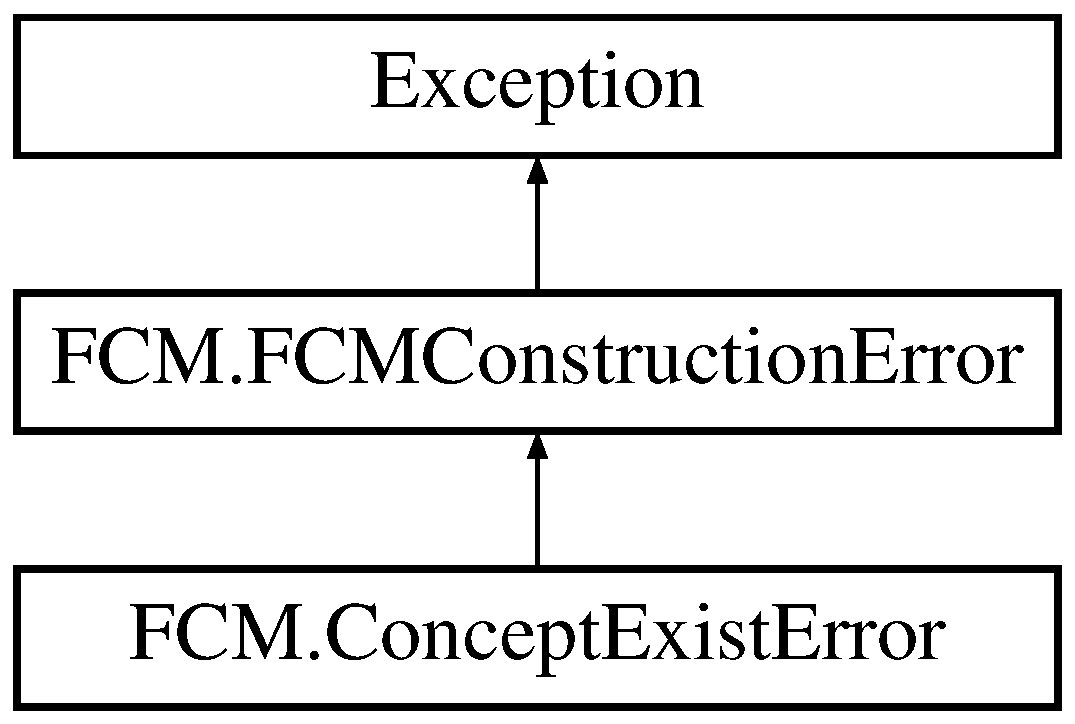
\includegraphics[height=3.000000cm]{class_f_c_m_1_1_concept_exist_error}
\end{center}
\end{figure}
\subsection*{Public Member Functions}
\begin{DoxyCompactItemize}
\item 
\hypertarget{class_f_c_m_1_1_concept_exist_error_ae367be09252d2594b59a659afac8a6da}{}\label{class_f_c_m_1_1_concept_exist_error_ae367be09252d2594b59a659afac8a6da} 
def {\bfseries \+\_\+\+\_\+init\+\_\+\+\_\+} (self, errors, message=\char`\"{}Concept does not exist \char`\"{})
\end{DoxyCompactItemize}


\subsection{Detailed Description}
\begin{DoxyVerb}This class is an exception class for Invalid concepts for the FCM
\end{DoxyVerb}
 

The documentation for this class was generated from the following file\+:\begin{DoxyCompactItemize}
\item 
F\+C\+M.\+py\end{DoxyCompactItemize}

\hypertarget{class_f_c_m_1_1_edge_exist_error}{}\section{F\+C\+M.\+Edge\+Exist\+Error Class Reference}
\label{class_f_c_m_1_1_edge_exist_error}\index{F\+C\+M.\+Edge\+Exist\+Error@{F\+C\+M.\+Edge\+Exist\+Error}}
Inheritance diagram for F\+C\+M.\+Edge\+Exist\+Error\+:\begin{figure}[H]
\begin{center}
\leavevmode
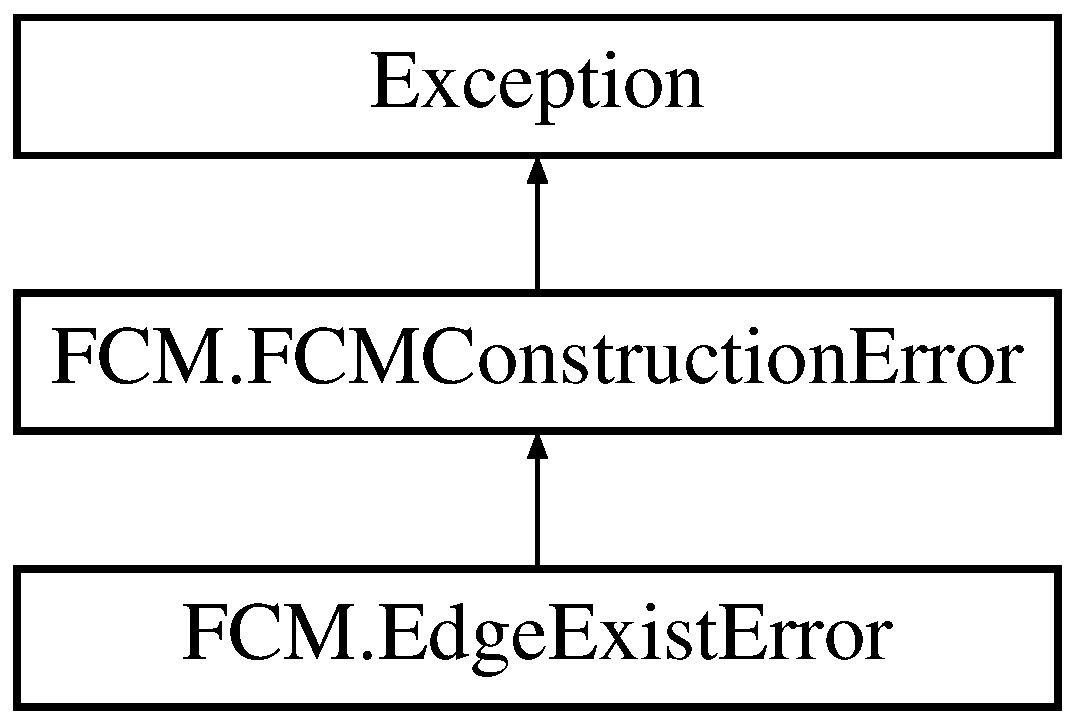
\includegraphics[height=3.000000cm]{class_f_c_m_1_1_edge_exist_error}
\end{center}
\end{figure}
\subsection*{Public Member Functions}
\begin{DoxyCompactItemize}
\item 
\hypertarget{class_f_c_m_1_1_edge_exist_error_aa7e4597cfa49f631e9fdcad821c02aed}{}\label{class_f_c_m_1_1_edge_exist_error_aa7e4597cfa49f631e9fdcad821c02aed} 
def {\bfseries \+\_\+\+\_\+init\+\_\+\+\_\+} (self, errors, message=\char`\"{}Edge does not exist between \char`\"{})
\end{DoxyCompactItemize}


\subsection{Detailed Description}
\begin{DoxyVerb}This class is an exception class for edge existence in FCM
\end{DoxyVerb}
 

The documentation for this class was generated from the following file\+:\begin{DoxyCompactItemize}
\item 
F\+C\+M.\+py\end{DoxyCompactItemize}

\hypertarget{class_f_c_m_1_1_f_c_m}{}\section{F\+C\+M.\+F\+CM Class Reference}
\label{class_f_c_m_1_1_f_c_m}\index{F\+C\+M.\+F\+CM@{F\+C\+M.\+F\+CM}}
\subsection*{Public Member Functions}
\begin{DoxyCompactItemize}
\item 
def \hyperlink{class_f_c_m_1_1_f_c_m_aba98e39a31a4bd9cb8eb8887dd98bbc0}{\+\_\+\+\_\+init\+\_\+\+\_\+} (self)
\item 
def \hyperlink{class_f_c_m_1_1_f_c_m_a57dff35d123327af6d02f335a49c4177}{add\+\_\+concept} (self, concept)
\item 
def \hyperlink{class_f_c_m_1_1_f_c_m_a4e32ab9228e8f678e6892092d643062d}{add\+\_\+edge} (self, concept1, concept2, weight)
\item 
def \hyperlink{class_f_c_m_1_1_f_c_m_a619a5925ca824a4e633378e2ceeca1fd}{get\+\_\+weight} (self, concept1, concept2)
\item 
def \hyperlink{class_f_c_m_1_1_f_c_m_a672188f630f4a42d330f7dc967933054}{remove\+\_\+edge} (self, node1, node2)
\item 
def \hyperlink{class_f_c_m_1_1_f_c_m_afcc0b9388e36ebe07b5b3b6c6d877a05}{remove\+\_\+concept} (self, concept)
\item 
def \hyperlink{class_f_c_m_1_1_f_c_m_abd95880fc46feca8042343b1556b61f1}{concepts} (self)
\item 
def \hyperlink{class_f_c_m_1_1_f_c_m_a55a0daf5c9eecef4639bb15ded281aa5}{set\+\_\+value} (self, concept, num)
\item 
def \hyperlink{class_f_c_m_1_1_f_c_m_ae764998f2c68740a4e80de8104da992d}{get\+\_\+concept\+\_\+value} (self, concept)
\item 
def \hyperlink{class_f_c_m_1_1_f_c_m_a97f12131aafc3d810da3ff95fb69ae1d}{draw} (self)
\end{DoxyCompactItemize}


\subsection{Detailed Description}
\begin{DoxyVerb}@package docstring
This is a Python class  for Fuzzy Cognitive Maps\end{DoxyVerb}
 

\subsection{Constructor \& Destructor Documentation}
\hypertarget{class_f_c_m_1_1_f_c_m_aba98e39a31a4bd9cb8eb8887dd98bbc0}{}\label{class_f_c_m_1_1_f_c_m_aba98e39a31a4bd9cb8eb8887dd98bbc0} 
\index{F\+C\+M\+::\+F\+CM@{F\+C\+M\+::\+F\+CM}!\+\_\+\+\_\+init\+\_\+\+\_\+@{\+\_\+\+\_\+init\+\_\+\+\_\+}}
\index{\+\_\+\+\_\+init\+\_\+\+\_\+@{\+\_\+\+\_\+init\+\_\+\+\_\+}!F\+C\+M\+::\+F\+CM@{F\+C\+M\+::\+F\+CM}}
\subsubsection{\texorpdfstring{\+\_\+\+\_\+init\+\_\+\+\_\+()}{\_\_init\_\_()}}
{\footnotesize\ttfamily def F\+C\+M.\+F\+C\+M.\+\_\+\+\_\+init\+\_\+\+\_\+ (\begin{DoxyParamCaption}\item[{}]{self }\end{DoxyParamCaption})}

\begin{DoxyVerb}@brief  This is the constructor for the Fuzzy graph.It initializes the networkx Digraph
@params none
\end{DoxyVerb}
 

\subsection{Member Function Documentation}
\hypertarget{class_f_c_m_1_1_f_c_m_a57dff35d123327af6d02f335a49c4177}{}\label{class_f_c_m_1_1_f_c_m_a57dff35d123327af6d02f335a49c4177} 
\index{F\+C\+M\+::\+F\+CM@{F\+C\+M\+::\+F\+CM}!add\+\_\+concept@{add\+\_\+concept}}
\index{add\+\_\+concept@{add\+\_\+concept}!F\+C\+M\+::\+F\+CM@{F\+C\+M\+::\+F\+CM}}
\subsubsection{\texorpdfstring{add\+\_\+concept()}{add\_concept()}}
{\footnotesize\ttfamily def F\+C\+M.\+F\+C\+M.\+add\+\_\+concept (\begin{DoxyParamCaption}\item[{}]{self,  }\item[{}]{concept }\end{DoxyParamCaption})}

\begin{DoxyVerb}@brief This method is an interface for the add_node method of DiGraph
@param concept A valid concept\end{DoxyVerb}
 \hypertarget{class_f_c_m_1_1_f_c_m_a4e32ab9228e8f678e6892092d643062d}{}\label{class_f_c_m_1_1_f_c_m_a4e32ab9228e8f678e6892092d643062d} 
\index{F\+C\+M\+::\+F\+CM@{F\+C\+M\+::\+F\+CM}!add\+\_\+edge@{add\+\_\+edge}}
\index{add\+\_\+edge@{add\+\_\+edge}!F\+C\+M\+::\+F\+CM@{F\+C\+M\+::\+F\+CM}}
\subsubsection{\texorpdfstring{add\+\_\+edge()}{add\_edge()}}
{\footnotesize\ttfamily def F\+C\+M.\+F\+C\+M.\+add\+\_\+edge (\begin{DoxyParamCaption}\item[{}]{self,  }\item[{}]{concept1,  }\item[{}]{concept2,  }\item[{}]{weight }\end{DoxyParamCaption})}

\begin{DoxyVerb}@brief This method is an interface for the add_edge method of Digraph.It checks whether the weight provided is the range of [-1,1].If the node does not exist,we create them before creating the edge.
@param concept1 a valid concept
@param concept2 a valid concept
@param weight a desired weight for the edge
\end{DoxyVerb}
 \hypertarget{class_f_c_m_1_1_f_c_m_abd95880fc46feca8042343b1556b61f1}{}\label{class_f_c_m_1_1_f_c_m_abd95880fc46feca8042343b1556b61f1} 
\index{F\+C\+M\+::\+F\+CM@{F\+C\+M\+::\+F\+CM}!concepts@{concepts}}
\index{concepts@{concepts}!F\+C\+M\+::\+F\+CM@{F\+C\+M\+::\+F\+CM}}
\subsubsection{\texorpdfstring{concepts()}{concepts()}}
{\footnotesize\ttfamily def F\+C\+M.\+F\+C\+M.\+concepts (\begin{DoxyParamCaption}\item[{}]{self }\end{DoxyParamCaption})}

\begin{DoxyVerb}@brief This method is an interface for nodes().It returns the dictionary of concepts in the graph having the node of the value as value and the concept as the key.
@param none
\end{DoxyVerb}
 \hypertarget{class_f_c_m_1_1_f_c_m_a97f12131aafc3d810da3ff95fb69ae1d}{}\label{class_f_c_m_1_1_f_c_m_a97f12131aafc3d810da3ff95fb69ae1d} 
\index{F\+C\+M\+::\+F\+CM@{F\+C\+M\+::\+F\+CM}!draw@{draw}}
\index{draw@{draw}!F\+C\+M\+::\+F\+CM@{F\+C\+M\+::\+F\+CM}}
\subsubsection{\texorpdfstring{draw()}{draw()}}
{\footnotesize\ttfamily def F\+C\+M.\+F\+C\+M.\+draw (\begin{DoxyParamCaption}\item[{}]{self }\end{DoxyParamCaption})}

\begin{DoxyVerb} @brief    This method is an interface for the draw() in the networkx package.We draw the DiGraph using spring layout and labels with the help of matplotlib
 @param none
\end{DoxyVerb}
 \hypertarget{class_f_c_m_1_1_f_c_m_ae764998f2c68740a4e80de8104da992d}{}\label{class_f_c_m_1_1_f_c_m_ae764998f2c68740a4e80de8104da992d} 
\index{F\+C\+M\+::\+F\+CM@{F\+C\+M\+::\+F\+CM}!get\+\_\+concept\+\_\+value@{get\+\_\+concept\+\_\+value}}
\index{get\+\_\+concept\+\_\+value@{get\+\_\+concept\+\_\+value}!F\+C\+M\+::\+F\+CM@{F\+C\+M\+::\+F\+CM}}
\subsubsection{\texorpdfstring{get\+\_\+concept\+\_\+value()}{get\_concept\_value()}}
{\footnotesize\ttfamily def F\+C\+M.\+F\+C\+M.\+get\+\_\+concept\+\_\+value (\begin{DoxyParamCaption}\item[{}]{self,  }\item[{}]{concept }\end{DoxyParamCaption})}

\begin{DoxyVerb}@brief returns the value of the concept
@param concept a valid concept
\end{DoxyVerb}
 \hypertarget{class_f_c_m_1_1_f_c_m_a619a5925ca824a4e633378e2ceeca1fd}{}\label{class_f_c_m_1_1_f_c_m_a619a5925ca824a4e633378e2ceeca1fd} 
\index{F\+C\+M\+::\+F\+CM@{F\+C\+M\+::\+F\+CM}!get\+\_\+weight@{get\+\_\+weight}}
\index{get\+\_\+weight@{get\+\_\+weight}!F\+C\+M\+::\+F\+CM@{F\+C\+M\+::\+F\+CM}}
\subsubsection{\texorpdfstring{get\+\_\+weight()}{get\_weight()}}
{\footnotesize\ttfamily def F\+C\+M.\+F\+C\+M.\+get\+\_\+weight (\begin{DoxyParamCaption}\item[{}]{self,  }\item[{}]{concept1,  }\item[{}]{concept2 }\end{DoxyParamCaption})}

\begin{DoxyVerb}@brief returns the weight of the edge,if the edge exists
@param concept1 a valid concept
@param concept2 a valid concept
\end{DoxyVerb}
 \hypertarget{class_f_c_m_1_1_f_c_m_afcc0b9388e36ebe07b5b3b6c6d877a05}{}\label{class_f_c_m_1_1_f_c_m_afcc0b9388e36ebe07b5b3b6c6d877a05} 
\index{F\+C\+M\+::\+F\+CM@{F\+C\+M\+::\+F\+CM}!remove\+\_\+concept@{remove\+\_\+concept}}
\index{remove\+\_\+concept@{remove\+\_\+concept}!F\+C\+M\+::\+F\+CM@{F\+C\+M\+::\+F\+CM}}
\subsubsection{\texorpdfstring{remove\+\_\+concept()}{remove\_concept()}}
{\footnotesize\ttfamily def F\+C\+M.\+F\+C\+M.\+remove\+\_\+concept (\begin{DoxyParamCaption}\item[{}]{self,  }\item[{}]{concept }\end{DoxyParamCaption})}

\begin{DoxyVerb}@brief This method is an interface for the remove_node() .If the node does exist,it prints an error message and returns.
@param concept A valid concept
\end{DoxyVerb}
 \hypertarget{class_f_c_m_1_1_f_c_m_a672188f630f4a42d330f7dc967933054}{}\label{class_f_c_m_1_1_f_c_m_a672188f630f4a42d330f7dc967933054} 
\index{F\+C\+M\+::\+F\+CM@{F\+C\+M\+::\+F\+CM}!remove\+\_\+edge@{remove\+\_\+edge}}
\index{remove\+\_\+edge@{remove\+\_\+edge}!F\+C\+M\+::\+F\+CM@{F\+C\+M\+::\+F\+CM}}
\subsubsection{\texorpdfstring{remove\+\_\+edge()}{remove\_edge()}}
{\footnotesize\ttfamily def F\+C\+M.\+F\+C\+M.\+remove\+\_\+edge (\begin{DoxyParamCaption}\item[{}]{self,  }\item[{}]{node1,  }\item[{}]{node2 }\end{DoxyParamCaption})}

\begin{DoxyVerb}@brief This method removes edges from the fcm graph.It also checks if the nodes exist and if the edge exists.
@param node1 a valid concept
@param node2 a valid concept
\end{DoxyVerb}
 \hypertarget{class_f_c_m_1_1_f_c_m_a55a0daf5c9eecef4639bb15ded281aa5}{}\label{class_f_c_m_1_1_f_c_m_a55a0daf5c9eecef4639bb15ded281aa5} 
\index{F\+C\+M\+::\+F\+CM@{F\+C\+M\+::\+F\+CM}!set\+\_\+value@{set\+\_\+value}}
\index{set\+\_\+value@{set\+\_\+value}!F\+C\+M\+::\+F\+CM@{F\+C\+M\+::\+F\+CM}}
\subsubsection{\texorpdfstring{set\+\_\+value()}{set\_value()}}
{\footnotesize\ttfamily def F\+C\+M.\+F\+C\+M.\+set\+\_\+value (\begin{DoxyParamCaption}\item[{}]{self,  }\item[{}]{concept,  }\item[{}]{num }\end{DoxyParamCaption})}

\begin{DoxyVerb}@brief This method adds an attribute to a node and accepts either an integer of a function which returns an integer
@param concept A valid concept
@param num a valid integer between [-1,1 ]
\end{DoxyVerb}
 

The documentation for this class was generated from the following file\+:\begin{DoxyCompactItemize}
\item 
F\+C\+M.\+py\end{DoxyCompactItemize}

\hypertarget{class_f_c_m_1_1_f_c_m_construction_error}{}\section{F\+C\+M.\+F\+C\+M\+Construction\+Error Class Reference}
\label{class_f_c_m_1_1_f_c_m_construction_error}\index{F\+C\+M.\+F\+C\+M\+Construction\+Error@{F\+C\+M.\+F\+C\+M\+Construction\+Error}}
Inheritance diagram for F\+C\+M.\+F\+C\+M\+Construction\+Error\+:\begin{figure}[H]
\begin{center}
\leavevmode
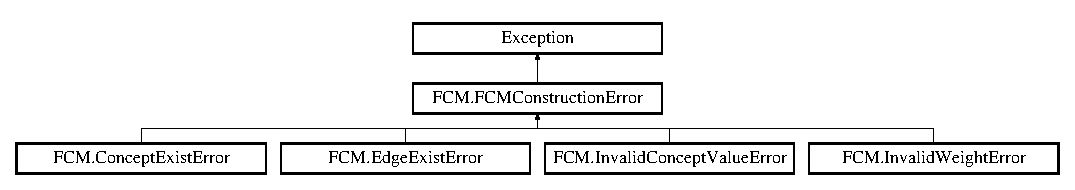
\includegraphics[height=2.110553cm]{class_f_c_m_1_1_f_c_m_construction_error}
\end{center}
\end{figure}
\subsection*{Public Member Functions}
\begin{DoxyCompactItemize}
\item 
\hypertarget{class_f_c_m_1_1_f_c_m_construction_error_a843bdbfe3b6d66d7b84b86bc1990c691}{}\label{class_f_c_m_1_1_f_c_m_construction_error_a843bdbfe3b6d66d7b84b86bc1990c691} 
def {\bfseries \+\_\+\+\_\+init\+\_\+\+\_\+} (self, message, errors)
\end{DoxyCompactItemize}


\subsection{Detailed Description}
\begin{DoxyVerb}This class is an exception for FCM construction error
\end{DoxyVerb}
 

The documentation for this class was generated from the following file\+:\begin{DoxyCompactItemize}
\item 
F\+C\+M.\+py\end{DoxyCompactItemize}

\hypertarget{class_f_c_m_1_1_invalid_concept_value_error}{}\section{F\+C\+M.\+Invalid\+Concept\+Value\+Error Class Reference}
\label{class_f_c_m_1_1_invalid_concept_value_error}\index{F\+C\+M.\+Invalid\+Concept\+Value\+Error@{F\+C\+M.\+Invalid\+Concept\+Value\+Error}}
Inheritance diagram for F\+C\+M.\+Invalid\+Concept\+Value\+Error\+:\begin{figure}[H]
\begin{center}
\leavevmode
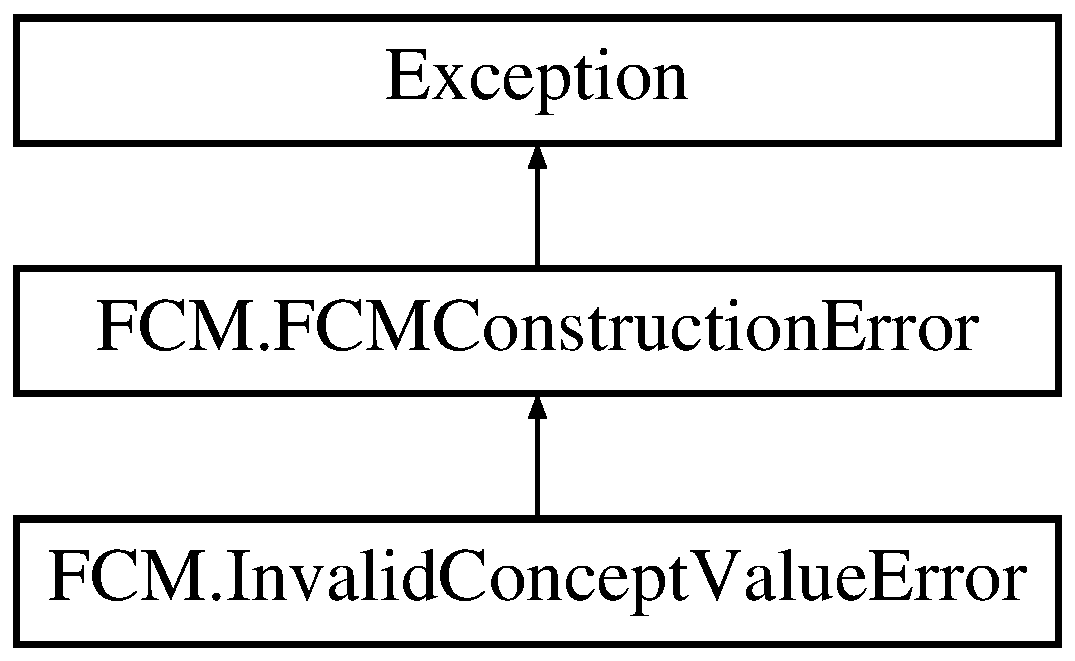
\includegraphics[height=3.000000cm]{class_f_c_m_1_1_invalid_concept_value_error}
\end{center}
\end{figure}
\subsection*{Public Member Functions}
\begin{DoxyCompactItemize}
\item 
\hypertarget{class_f_c_m_1_1_invalid_concept_value_error_abb1b2a8b8c9d1c8b335e392c228ee805}{}\label{class_f_c_m_1_1_invalid_concept_value_error_abb1b2a8b8c9d1c8b335e392c228ee805} 
def {\bfseries \+\_\+\+\_\+init\+\_\+\+\_\+} (self, errors, message=\char`\"{}Invalid Concept value \char`\"{})
\end{DoxyCompactItemize}


\subsection{Detailed Description}
\begin{DoxyVerb}This class is an exception class for invalid concept value of FCM
\end{DoxyVerb}
 

The documentation for this class was generated from the following file\+:\begin{DoxyCompactItemize}
\item 
F\+C\+M.\+py\end{DoxyCompactItemize}

\hypertarget{class_f_c_m_1_1_invalid_weight_error}{}\section{F\+C\+M.\+Invalid\+Weight\+Error Class Reference}
\label{class_f_c_m_1_1_invalid_weight_error}\index{F\+C\+M.\+Invalid\+Weight\+Error@{F\+C\+M.\+Invalid\+Weight\+Error}}
Inheritance diagram for F\+C\+M.\+Invalid\+Weight\+Error\+:\begin{figure}[H]
\begin{center}
\leavevmode
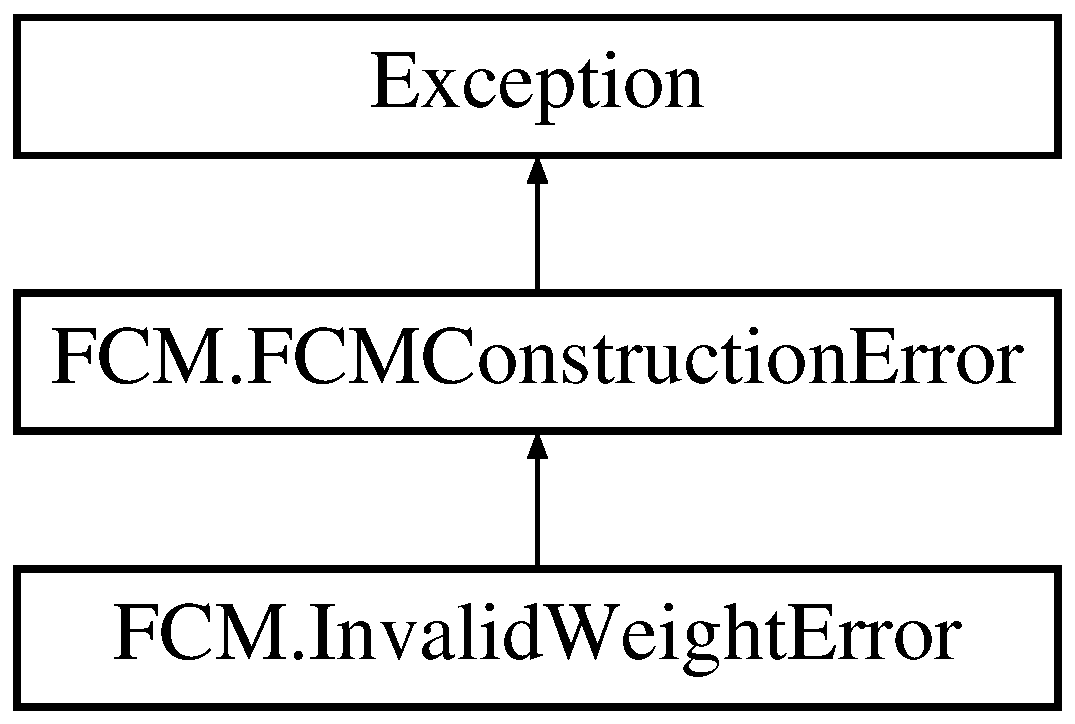
\includegraphics[height=3.000000cm]{class_f_c_m_1_1_invalid_weight_error}
\end{center}
\end{figure}
\subsection*{Public Member Functions}
\begin{DoxyCompactItemize}
\item 
\hypertarget{class_f_c_m_1_1_invalid_weight_error_a0727a96acad375593fb2e619fddce1ba}{}\label{class_f_c_m_1_1_invalid_weight_error_a0727a96acad375593fb2e619fddce1ba} 
def {\bfseries \+\_\+\+\_\+init\+\_\+\+\_\+} (self, errors, message=\char`\"{}Invalid weight for an edge \char`\"{})
\end{DoxyCompactItemize}


\subsection{Detailed Description}
\begin{DoxyVerb}This class is an exception class for Invalid weights for FCM edges
\end{DoxyVerb}
 

The documentation for this class was generated from the following file\+:\begin{DoxyCompactItemize}
\item 
F\+C\+M.\+py\end{DoxyCompactItemize}

\hypertarget{class_particle___swarm___optimization_1_1_p_s_o}{}\section{Particle\+\_\+\+Swarm\+\_\+\+Optimization.\+P\+SO Class Reference}
\label{class_particle___swarm___optimization_1_1_p_s_o}\index{Particle\+\_\+\+Swarm\+\_\+\+Optimization.\+P\+SO@{Particle\+\_\+\+Swarm\+\_\+\+Optimization.\+P\+SO}}
\subsection*{Public Member Functions}
\begin{DoxyCompactItemize}
\item 
def \hyperlink{class_particle___swarm___optimization_1_1_p_s_o_add702c734a63162dbe1cbfd6f94f26f7}{\+\_\+\+\_\+init\+\_\+\+\_\+} (self, fcm, converge\+\_\+concepts\+\_\+dict, steepness\+\_\+parameter=1, max\+\_\+iterations=10, constriction\+\_\+factor=0.\+7, cognitive\+\_\+parameter=2, social\+\_\+parameter=2)
\item 
def \hyperlink{class_particle___swarm___optimization_1_1_p_s_o_a8cfda07a7b320a55112993aea3a1f921}{sigmoid} (self, x)
\item 
def \hyperlink{class_particle___swarm___optimization_1_1_p_s_o_a923072a9af1fea8affadfd0bd1a947cf}{heaviside} (self, x)
\item 
def \hyperlink{class_particle___swarm___optimization_1_1_p_s_o_a88adc64e6121ec070e2736145edabd4c}{initialize\+\_\+weight\+\_\+matrix} (self)
\item 
def \hyperlink{class_particle___swarm___optimization_1_1_p_s_o_abf63d69aa42e75058a939c6dac4416c5}{get\+\_\+updated\+\_\+concept\+\_\+values} (self, concept)
\item 
def \hyperlink{class_particle___swarm___optimization_1_1_p_s_o_aadc88450078ac4c483d890a87dee9b0e}{get\+\_\+fitness} (self, weight)
\item 
def \hyperlink{class_particle___swarm___optimization_1_1_p_s_o_a950b777176b42eb5b488c1b822cd0275}{schaffer\+F6\+Helper\+Function} (self, index, weight)
\item 
def \hyperlink{class_particle___swarm___optimization_1_1_p_s_o_aba0d1ce14ce74445ee798358d5475559}{get\+\_\+swarm\+\_\+weights} (self)
\item 
def \hyperlink{class_particle___swarm___optimization_1_1_p_s_o_a810301f0aeba3b2e31dd5c5203b8b201}{in\+\_\+bounds} (self, value, bounds)
\item 
def \hyperlink{class_particle___swarm___optimization_1_1_p_s_o_a26c6af0753a8c0508b2f3d1a727537a7}{check\+\_\+concept\+\_\+bounds} (self)
\item 
def \hyperlink{class_particle___swarm___optimization_1_1_p_s_o_a9a1612724d06d65b4046b5ff26cb9cef}{run\+\_\+convergence} (self)
\end{DoxyCompactItemize}
\subsection*{Public Attributes}
\begin{DoxyCompactItemize}
\item 
\hypertarget{class_particle___swarm___optimization_1_1_p_s_o_a5f47340d853921528588246d89909f3a}{}\label{class_particle___swarm___optimization_1_1_p_s_o_a5f47340d853921528588246d89909f3a} 
{\bfseries fcm}
\item 
\hypertarget{class_particle___swarm___optimization_1_1_p_s_o_aa07c49004eee002a18014fdee545c57e}{}\label{class_particle___swarm___optimization_1_1_p_s_o_aa07c49004eee002a18014fdee545c57e} 
{\bfseries converge\+\_\+concepts}
\item 
\hypertarget{class_particle___swarm___optimization_1_1_p_s_o_abbfe6efc1b6130b342ac8faaaa240fda}{}\label{class_particle___swarm___optimization_1_1_p_s_o_abbfe6efc1b6130b342ac8faaaa240fda} 
{\bfseries converge\+\_\+concepts\+\_\+dict}
\item 
\hypertarget{class_particle___swarm___optimization_1_1_p_s_o_aa97ec334df2394416c5feb90a561450a}{}\label{class_particle___swarm___optimization_1_1_p_s_o_aa97ec334df2394416c5feb90a561450a} 
{\bfseries steepness\+\_\+parameter}
\item 
\hypertarget{class_particle___swarm___optimization_1_1_p_s_o_a1dc7c802032c32533934070034773ea2}{}\label{class_particle___swarm___optimization_1_1_p_s_o_a1dc7c802032c32533934070034773ea2} 
{\bfseries weight\+\_\+matrix}
\item 
\hypertarget{class_particle___swarm___optimization_1_1_p_s_o_a07a935095fdf04234de7cc880c38a1aa}{}\label{class_particle___swarm___optimization_1_1_p_s_o_a07a935095fdf04234de7cc880c38a1aa} 
{\bfseries constriction\+\_\+factor}
\item 
\hypertarget{class_particle___swarm___optimization_1_1_p_s_o_a16bb4fbcbd469227d9430e2f33ba752a}{}\label{class_particle___swarm___optimization_1_1_p_s_o_a16bb4fbcbd469227d9430e2f33ba752a} 
{\bfseries cognitive\+\_\+parameter}
\item 
\hypertarget{class_particle___swarm___optimization_1_1_p_s_o_a79d6d507270c1873776cad9bf991581f}{}\label{class_particle___swarm___optimization_1_1_p_s_o_a79d6d507270c1873776cad9bf991581f} 
{\bfseries social\+\_\+parameter}
\item 
\hypertarget{class_particle___swarm___optimization_1_1_p_s_o_a0be7c542209de08c5f4a7a7f8b81fd91}{}\label{class_particle___swarm___optimization_1_1_p_s_o_a0be7c542209de08c5f4a7a7f8b81fd91} 
{\bfseries max\+\_\+iterations}
\item 
\hypertarget{class_particle___swarm___optimization_1_1_p_s_o_ae6a19613b5aaa8ec64fcf4b7c27743a1}{}\label{class_particle___swarm___optimization_1_1_p_s_o_ae6a19613b5aaa8ec64fcf4b7c27743a1} 
{\bfseries fitness\+\_\+list}
\item 
\hypertarget{class_particle___swarm___optimization_1_1_p_s_o_a04d287712fa8a98e8482dccf35dbc562}{}\label{class_particle___swarm___optimization_1_1_p_s_o_a04d287712fa8a98e8482dccf35dbc562} 
{\bfseries velocity\+\_\+list}
\item 
\hypertarget{class_particle___swarm___optimization_1_1_p_s_o_a079f0fb7cd69fde03cbe5409c9113cf7}{}\label{class_particle___swarm___optimization_1_1_p_s_o_a079f0fb7cd69fde03cbe5409c9113cf7} 
{\bfseries best\+\_\+weights}
\end{DoxyCompactItemize}


\subsection{Detailed Description}
\begin{DoxyVerb}This class is a class which runs the Particle Swarm Optimization for FCMs to make
sure that the concepts converge to the bounds given by the experts and the weights
are globally minimized.\end{DoxyVerb}
 

\subsection{Constructor \& Destructor Documentation}
\hypertarget{class_particle___swarm___optimization_1_1_p_s_o_add702c734a63162dbe1cbfd6f94f26f7}{}\label{class_particle___swarm___optimization_1_1_p_s_o_add702c734a63162dbe1cbfd6f94f26f7} 
\index{Particle\+\_\+\+Swarm\+\_\+\+Optimization\+::\+P\+SO@{Particle\+\_\+\+Swarm\+\_\+\+Optimization\+::\+P\+SO}!\+\_\+\+\_\+init\+\_\+\+\_\+@{\+\_\+\+\_\+init\+\_\+\+\_\+}}
\index{\+\_\+\+\_\+init\+\_\+\+\_\+@{\+\_\+\+\_\+init\+\_\+\+\_\+}!Particle\+\_\+\+Swarm\+\_\+\+Optimization\+::\+P\+SO@{Particle\+\_\+\+Swarm\+\_\+\+Optimization\+::\+P\+SO}}
\subsubsection{\texorpdfstring{\+\_\+\+\_\+init\+\_\+\+\_\+()}{\_\_init\_\_()}}
{\footnotesize\ttfamily def Particle\+\_\+\+Swarm\+\_\+\+Optimization.\+P\+S\+O.\+\_\+\+\_\+init\+\_\+\+\_\+ (\begin{DoxyParamCaption}\item[{}]{self,  }\item[{}]{fcm,  }\item[{}]{converge\+\_\+concepts\+\_\+dict,  }\item[{}]{steepness\+\_\+parameter = {\ttfamily 1},  }\item[{}]{max\+\_\+iterations = {\ttfamily 10},  }\item[{}]{constriction\+\_\+factor = {\ttfamily 0.7},  }\item[{}]{cognitive\+\_\+parameter = {\ttfamily 2},  }\item[{}]{social\+\_\+parameter = {\ttfamily 2} }\end{DoxyParamCaption})}

\begin{DoxyVerb}@brief : The constructor here initializes the required attributes which are necessary to run the algorithm .

@param : fcm - a valid FCM object
     converge concepts dictionary : a dictionary where the keys are concepts and value is the
     tuple describing its bounds. Example : {'Tank1' : (0.3,0.9),'Tank2' : '(0.2,0,7)'}

     the default parameters are steepness_parameter,max_iterations,constriction_factor,cognitive_parameter,
     social_parameter which are required for the algorithm\end{DoxyVerb}
 

\subsection{Member Function Documentation}
\hypertarget{class_particle___swarm___optimization_1_1_p_s_o_a26c6af0753a8c0508b2f3d1a727537a7}{}\label{class_particle___swarm___optimization_1_1_p_s_o_a26c6af0753a8c0508b2f3d1a727537a7} 
\index{Particle\+\_\+\+Swarm\+\_\+\+Optimization\+::\+P\+SO@{Particle\+\_\+\+Swarm\+\_\+\+Optimization\+::\+P\+SO}!check\+\_\+concept\+\_\+bounds@{check\+\_\+concept\+\_\+bounds}}
\index{check\+\_\+concept\+\_\+bounds@{check\+\_\+concept\+\_\+bounds}!Particle\+\_\+\+Swarm\+\_\+\+Optimization\+::\+P\+SO@{Particle\+\_\+\+Swarm\+\_\+\+Optimization\+::\+P\+SO}}
\subsubsection{\texorpdfstring{check\+\_\+concept\+\_\+bounds()}{check\_concept\_bounds()}}
{\footnotesize\ttfamily def Particle\+\_\+\+Swarm\+\_\+\+Optimization.\+P\+S\+O.\+check\+\_\+concept\+\_\+bounds (\begin{DoxyParamCaption}\item[{}]{self }\end{DoxyParamCaption})}

\begin{DoxyVerb}@brief: This method checks if the concepts are asked to be converged are within the given bounds or not.This function is the
    termination function for the algorithm
@param  : No parameters other than the self parameter
\end{DoxyVerb}
 \hypertarget{class_particle___swarm___optimization_1_1_p_s_o_aadc88450078ac4c483d890a87dee9b0e}{}\label{class_particle___swarm___optimization_1_1_p_s_o_aadc88450078ac4c483d890a87dee9b0e} 
\index{Particle\+\_\+\+Swarm\+\_\+\+Optimization\+::\+P\+SO@{Particle\+\_\+\+Swarm\+\_\+\+Optimization\+::\+P\+SO}!get\+\_\+fitness@{get\+\_\+fitness}}
\index{get\+\_\+fitness@{get\+\_\+fitness}!Particle\+\_\+\+Swarm\+\_\+\+Optimization\+::\+P\+SO@{Particle\+\_\+\+Swarm\+\_\+\+Optimization\+::\+P\+SO}}
\subsubsection{\texorpdfstring{get\+\_\+fitness()}{get\_fitness()}}
{\footnotesize\ttfamily def Particle\+\_\+\+Swarm\+\_\+\+Optimization.\+P\+S\+O.\+get\+\_\+fitness (\begin{DoxyParamCaption}\item[{}]{self,  }\item[{}]{weight }\end{DoxyParamCaption})}

\begin{DoxyVerb}@brief : It is an implementation of the schaffer F6 function which is used to calculate the fitness of the weights
@param weight - a valid weight number\end{DoxyVerb}
 \hypertarget{class_particle___swarm___optimization_1_1_p_s_o_aba0d1ce14ce74445ee798358d5475559}{}\label{class_particle___swarm___optimization_1_1_p_s_o_aba0d1ce14ce74445ee798358d5475559} 
\index{Particle\+\_\+\+Swarm\+\_\+\+Optimization\+::\+P\+SO@{Particle\+\_\+\+Swarm\+\_\+\+Optimization\+::\+P\+SO}!get\+\_\+swarm\+\_\+weights@{get\+\_\+swarm\+\_\+weights}}
\index{get\+\_\+swarm\+\_\+weights@{get\+\_\+swarm\+\_\+weights}!Particle\+\_\+\+Swarm\+\_\+\+Optimization\+::\+P\+SO@{Particle\+\_\+\+Swarm\+\_\+\+Optimization\+::\+P\+SO}}
\subsubsection{\texorpdfstring{get\+\_\+swarm\+\_\+weights()}{get\_swarm\_weights()}}
{\footnotesize\ttfamily def Particle\+\_\+\+Swarm\+\_\+\+Optimization.\+P\+S\+O.\+get\+\_\+swarm\+\_\+weights (\begin{DoxyParamCaption}\item[{}]{self }\end{DoxyParamCaption})}

\begin{DoxyVerb}@brief   This function is used to get the swarm weights by finding the
     global best and the local best and will update the weights
@param  This function takes no parameters other than the self parameter\end{DoxyVerb}
 \hypertarget{class_particle___swarm___optimization_1_1_p_s_o_abf63d69aa42e75058a939c6dac4416c5}{}\label{class_particle___swarm___optimization_1_1_p_s_o_abf63d69aa42e75058a939c6dac4416c5} 
\index{Particle\+\_\+\+Swarm\+\_\+\+Optimization\+::\+P\+SO@{Particle\+\_\+\+Swarm\+\_\+\+Optimization\+::\+P\+SO}!get\+\_\+updated\+\_\+concept\+\_\+values@{get\+\_\+updated\+\_\+concept\+\_\+values}}
\index{get\+\_\+updated\+\_\+concept\+\_\+values@{get\+\_\+updated\+\_\+concept\+\_\+values}!Particle\+\_\+\+Swarm\+\_\+\+Optimization\+::\+P\+SO@{Particle\+\_\+\+Swarm\+\_\+\+Optimization\+::\+P\+SO}}
\subsubsection{\texorpdfstring{get\+\_\+updated\+\_\+concept\+\_\+values()}{get\_updated\_concept\_values()}}
{\footnotesize\ttfamily def Particle\+\_\+\+Swarm\+\_\+\+Optimization.\+P\+S\+O.\+get\+\_\+updated\+\_\+concept\+\_\+values (\begin{DoxyParamCaption}\item[{}]{self,  }\item[{}]{concept }\end{DoxyParamCaption})}

\begin{DoxyVerb}@brief This function updates the concept values according to the changed weights
@param concept This function takes a valid concept as a parameter
\end{DoxyVerb}
 \hypertarget{class_particle___swarm___optimization_1_1_p_s_o_a923072a9af1fea8affadfd0bd1a947cf}{}\label{class_particle___swarm___optimization_1_1_p_s_o_a923072a9af1fea8affadfd0bd1a947cf} 
\index{Particle\+\_\+\+Swarm\+\_\+\+Optimization\+::\+P\+SO@{Particle\+\_\+\+Swarm\+\_\+\+Optimization\+::\+P\+SO}!heaviside@{heaviside}}
\index{heaviside@{heaviside}!Particle\+\_\+\+Swarm\+\_\+\+Optimization\+::\+P\+SO@{Particle\+\_\+\+Swarm\+\_\+\+Optimization\+::\+P\+SO}}
\subsubsection{\texorpdfstring{heaviside()}{heaviside()}}
{\footnotesize\ttfamily def Particle\+\_\+\+Swarm\+\_\+\+Optimization.\+P\+S\+O.\+heaviside (\begin{DoxyParamCaption}\item[{}]{self,  }\item[{}]{x }\end{DoxyParamCaption})}

\begin{DoxyVerb}@brief  This function is used to determine the objective function which acts as a global minimizer which returns either 0 or 1
@param  x  a valid integer
\end{DoxyVerb}
 \hypertarget{class_particle___swarm___optimization_1_1_p_s_o_a810301f0aeba3b2e31dd5c5203b8b201}{}\label{class_particle___swarm___optimization_1_1_p_s_o_a810301f0aeba3b2e31dd5c5203b8b201} 
\index{Particle\+\_\+\+Swarm\+\_\+\+Optimization\+::\+P\+SO@{Particle\+\_\+\+Swarm\+\_\+\+Optimization\+::\+P\+SO}!in\+\_\+bounds@{in\+\_\+bounds}}
\index{in\+\_\+bounds@{in\+\_\+bounds}!Particle\+\_\+\+Swarm\+\_\+\+Optimization\+::\+P\+SO@{Particle\+\_\+\+Swarm\+\_\+\+Optimization\+::\+P\+SO}}
\subsubsection{\texorpdfstring{in\+\_\+bounds()}{in\_bounds()}}
{\footnotesize\ttfamily def Particle\+\_\+\+Swarm\+\_\+\+Optimization.\+P\+S\+O.\+in\+\_\+bounds (\begin{DoxyParamCaption}\item[{}]{self,  }\item[{}]{value,  }\item[{}]{bounds }\end{DoxyParamCaption})}

\begin{DoxyVerb}@brief : This method is a utility function which is used to tell if the value lies between the bounds

@param : value - a valid integer
   bounds - a tuple in sorted ascending order\end{DoxyVerb}
 \hypertarget{class_particle___swarm___optimization_1_1_p_s_o_a88adc64e6121ec070e2736145edabd4c}{}\label{class_particle___swarm___optimization_1_1_p_s_o_a88adc64e6121ec070e2736145edabd4c} 
\index{Particle\+\_\+\+Swarm\+\_\+\+Optimization\+::\+P\+SO@{Particle\+\_\+\+Swarm\+\_\+\+Optimization\+::\+P\+SO}!initialize\+\_\+weight\+\_\+matrix@{initialize\+\_\+weight\+\_\+matrix}}
\index{initialize\+\_\+weight\+\_\+matrix@{initialize\+\_\+weight\+\_\+matrix}!Particle\+\_\+\+Swarm\+\_\+\+Optimization\+::\+P\+SO@{Particle\+\_\+\+Swarm\+\_\+\+Optimization\+::\+P\+SO}}
\subsubsection{\texorpdfstring{initialize\+\_\+weight\+\_\+matrix()}{initialize\_weight\_matrix()}}
{\footnotesize\ttfamily def Particle\+\_\+\+Swarm\+\_\+\+Optimization.\+P\+S\+O.\+initialize\+\_\+weight\+\_\+matrix (\begin{DoxyParamCaption}\item[{}]{self }\end{DoxyParamCaption})}

\begin{DoxyVerb}@brief : This function is used to create a dictionary of dictionary of the weights of the concept edges
@param : This function takes no parameters other than the self parameter
\end{DoxyVerb}
 \hypertarget{class_particle___swarm___optimization_1_1_p_s_o_a9a1612724d06d65b4046b5ff26cb9cef}{}\label{class_particle___swarm___optimization_1_1_p_s_o_a9a1612724d06d65b4046b5ff26cb9cef} 
\index{Particle\+\_\+\+Swarm\+\_\+\+Optimization\+::\+P\+SO@{Particle\+\_\+\+Swarm\+\_\+\+Optimization\+::\+P\+SO}!run\+\_\+convergence@{run\+\_\+convergence}}
\index{run\+\_\+convergence@{run\+\_\+convergence}!Particle\+\_\+\+Swarm\+\_\+\+Optimization\+::\+P\+SO@{Particle\+\_\+\+Swarm\+\_\+\+Optimization\+::\+P\+SO}}
\subsubsection{\texorpdfstring{run\+\_\+convergence()}{run\_convergence()}}
{\footnotesize\ttfamily def Particle\+\_\+\+Swarm\+\_\+\+Optimization.\+P\+S\+O.\+run\+\_\+convergence (\begin{DoxyParamCaption}\item[{}]{self }\end{DoxyParamCaption})}

\begin{DoxyVerb}@brief : This function runs the algorithm which changes the convergence
         algorithm by the following steps :
         1) Initialize the weight matrix
         2) For the requested concepts ,check if they are in bounds,
         3) If they are out of bounds,do the following
         4) Run the swarm for weight matrix
         5) Calculate the objective function
         6) If the concept values converge,stop the algorithm
         7) Else,continue the process

@param  : This method takes no parameters other than the self parameter\end{DoxyVerb}
 \hypertarget{class_particle___swarm___optimization_1_1_p_s_o_a950b777176b42eb5b488c1b822cd0275}{}\label{class_particle___swarm___optimization_1_1_p_s_o_a950b777176b42eb5b488c1b822cd0275} 
\index{Particle\+\_\+\+Swarm\+\_\+\+Optimization\+::\+P\+SO@{Particle\+\_\+\+Swarm\+\_\+\+Optimization\+::\+P\+SO}!schaffer\+F6\+Helper\+Function@{schaffer\+F6\+Helper\+Function}}
\index{schaffer\+F6\+Helper\+Function@{schaffer\+F6\+Helper\+Function}!Particle\+\_\+\+Swarm\+\_\+\+Optimization\+::\+P\+SO@{Particle\+\_\+\+Swarm\+\_\+\+Optimization\+::\+P\+SO}}
\subsubsection{\texorpdfstring{schaffer\+F6\+Helper\+Function()}{schafferF6HelperFunction()}}
{\footnotesize\ttfamily def Particle\+\_\+\+Swarm\+\_\+\+Optimization.\+P\+S\+O.\+schaffer\+F6\+Helper\+Function (\begin{DoxyParamCaption}\item[{}]{self,  }\item[{}]{index,  }\item[{}]{weight }\end{DoxyParamCaption})}

\begin{DoxyVerb}@brief  This function is a pairwise schaffer F6 calculator which is used by the above function
    The formula is 0.5 + (sin(sqrt(x**2+y**2))-0.5) /(1+0.001*(x**2+y**2))**2
@param index - a valid integer
   weight - a valid weight\end{DoxyVerb}
 \hypertarget{class_particle___swarm___optimization_1_1_p_s_o_a8cfda07a7b320a55112993aea3a1f921}{}\label{class_particle___swarm___optimization_1_1_p_s_o_a8cfda07a7b320a55112993aea3a1f921} 
\index{Particle\+\_\+\+Swarm\+\_\+\+Optimization\+::\+P\+SO@{Particle\+\_\+\+Swarm\+\_\+\+Optimization\+::\+P\+SO}!sigmoid@{sigmoid}}
\index{sigmoid@{sigmoid}!Particle\+\_\+\+Swarm\+\_\+\+Optimization\+::\+P\+SO@{Particle\+\_\+\+Swarm\+\_\+\+Optimization\+::\+P\+SO}}
\subsubsection{\texorpdfstring{sigmoid()}{sigmoid()}}
{\footnotesize\ttfamily def Particle\+\_\+\+Swarm\+\_\+\+Optimization.\+P\+S\+O.\+sigmoid (\begin{DoxyParamCaption}\item[{}]{self,  }\item[{}]{x }\end{DoxyParamCaption})}

\begin{DoxyVerb}@brief The formula is  f(x)=(1)(1+exp(-x))
@param x - a valid integer\end{DoxyVerb}
 

The documentation for this class was generated from the following file\+:\begin{DoxyCompactItemize}
\item 
Particle\+\_\+\+Swarm\+\_\+\+Optimization.\+py\end{DoxyCompactItemize}

\hypertarget{class_simulation_1_1simulation}{}\section{Simulation.\+simulation Class Reference}
\label{class_simulation_1_1simulation}\index{Simulation.\+simulation@{Simulation.\+simulation}}
\subsection*{Public Member Functions}
\begin{DoxyCompactItemize}
\item 
def \hyperlink{class_simulation_1_1simulation_a0f0377da7ec6ea298232042744c03e89}{\+\_\+\+\_\+init\+\_\+\+\_\+} (self, \hyperlink{class_f_c_m_1_1_f_c_m}{F\+CM}, converge\+\_\+concepts\+\_\+dict)
\item 
def \hyperlink{class_simulation_1_1simulation_aba88676dbf04c07845b65cae2c85e536}{stabilize} (self, concept, threshold)
\item 
def \hyperlink{class_simulation_1_1simulation_ae4ffda917687b0cb3cd1582e15e7541d}{steps} (self, numsteps)
\item 
def \hyperlink{class_simulation_1_1simulation_a6de2037ab28f1fd076cadeb95f1e83fa}{change\+Transfer\+Function} (self, function)
\item 
def \hyperlink{class_simulation_1_1simulation_a2f32f5da01e7f1485510f5982be2860c}{run} (self, run\+\_\+particle\+\_\+swarm=False, c=None)
\end{DoxyCompactItemize}
\subsection*{Public Attributes}
\begin{DoxyCompactItemize}
\item 
\hypertarget{class_simulation_1_1simulation_a671846c113f0a9dc83286c5ad9512285}{}\label{class_simulation_1_1simulation_a671846c113f0a9dc83286c5ad9512285} 
{\bfseries fcm}
\item 
\hypertarget{class_simulation_1_1simulation_a868424f7c18c88721f794fa099eadec7}{}\label{class_simulation_1_1simulation_a868424f7c18c88721f794fa099eadec7} 
{\bfseries num\+Steps}
\item 
\hypertarget{class_simulation_1_1simulation_aec4266415db730e604fd19efd35bef84}{}\label{class_simulation_1_1simulation_aec4266415db730e604fd19efd35bef84} 
{\bfseries stabilizers}
\item 
\hypertarget{class_simulation_1_1simulation_af0a20076b369e7b1917db3dcd5b77f60}{}\label{class_simulation_1_1simulation_af0a20076b369e7b1917db3dcd5b77f60} 
{\bfseries stable\+Dict}
\item 
\hypertarget{class_simulation_1_1simulation_a0bf335dc7d60b29f151285ebfca3e665}{}\label{class_simulation_1_1simulation_a0bf335dc7d60b29f151285ebfca3e665} 
{\bfseries transfer\+Function}
\item 
\hypertarget{class_simulation_1_1simulation_a90288804c2a984095032eac0218bf92b}{}\label{class_simulation_1_1simulation_a90288804c2a984095032eac0218bf92b} 
{\bfseries edge\+Matrix}
\item 
\hypertarget{class_simulation_1_1simulation_a3c3e4f6c4750204ae65db87b36bd3533}{}\label{class_simulation_1_1simulation_a3c3e4f6c4750204ae65db87b36bd3533} 
{\bfseries stable\+\_\+concepts}
\end{DoxyCompactItemize}


\subsection{Detailed Description}
\begin{DoxyVerb}This class is responsible for the simulation of the Fuzzy Cognitive Maps.
It has a method called 'run()' which can run both Regular Simulation as
well as the Particle Swarm Optimization with the help of an optional parameter\end{DoxyVerb}
 

\subsection{Constructor \& Destructor Documentation}
\hypertarget{class_simulation_1_1simulation_a0f0377da7ec6ea298232042744c03e89}{}\label{class_simulation_1_1simulation_a0f0377da7ec6ea298232042744c03e89} 
\index{Simulation\+::simulation@{Simulation\+::simulation}!\+\_\+\+\_\+init\+\_\+\+\_\+@{\+\_\+\+\_\+init\+\_\+\+\_\+}}
\index{\+\_\+\+\_\+init\+\_\+\+\_\+@{\+\_\+\+\_\+init\+\_\+\+\_\+}!Simulation\+::simulation@{Simulation\+::simulation}}
\subsubsection{\texorpdfstring{\+\_\+\+\_\+init\+\_\+\+\_\+()}{\_\_init\_\_()}}
{\footnotesize\ttfamily def Simulation.\+simulation.\+\_\+\+\_\+init\+\_\+\+\_\+ (\begin{DoxyParamCaption}\item[{}]{self,  }\item[{}]{F\+CM,  }\item[{}]{converge\+\_\+concepts\+\_\+dict }\end{DoxyParamCaption})}

\begin{DoxyVerb}Constructor
The constructor takes the following parameters
1) FCM object
2) a dictionary with key as concept and value as a tuple of size 2
\end{DoxyVerb}
\begin{DoxyVerb}an fcm object \end{DoxyVerb}
 

\subsection{Member Function Documentation}
\hypertarget{class_simulation_1_1simulation_a6de2037ab28f1fd076cadeb95f1e83fa}{}\label{class_simulation_1_1simulation_a6de2037ab28f1fd076cadeb95f1e83fa} 
\index{Simulation\+::simulation@{Simulation\+::simulation}!change\+Transfer\+Function@{change\+Transfer\+Function}}
\index{change\+Transfer\+Function@{change\+Transfer\+Function}!Simulation\+::simulation@{Simulation\+::simulation}}
\subsubsection{\texorpdfstring{change\+Transfer\+Function()}{changeTransferFunction()}}
{\footnotesize\ttfamily def Simulation.\+simulation.\+change\+Transfer\+Function (\begin{DoxyParamCaption}\item[{}]{self,  }\item[{}]{function }\end{DoxyParamCaption})}

\begin{DoxyVerb}changeTransferFunction
Parameters: function (function with 1 argument): a function that takes one argument and maintains values in range [-1,1]
return: void
Description: Changes the transfer function. error check will pass 100 and -100  to see if they stay in range
\end{DoxyVerb}
 \hypertarget{class_simulation_1_1simulation_a2f32f5da01e7f1485510f5982be2860c}{}\label{class_simulation_1_1simulation_a2f32f5da01e7f1485510f5982be2860c} 
\index{Simulation\+::simulation@{Simulation\+::simulation}!run@{run}}
\index{run@{run}!Simulation\+::simulation@{Simulation\+::simulation}}
\subsubsection{\texorpdfstring{run()}{run()}}
{\footnotesize\ttfamily def Simulation.\+simulation.\+run (\begin{DoxyParamCaption}\item[{}]{self,  }\item[{}]{run\+\_\+particle\+\_\+swarm = {\ttfamily False},  }\item[{}]{c = {\ttfamily None} }\end{DoxyParamCaption})}

\begin{DoxyVerb}Run
Arguments: c (optional): weight for the nodes to be adjusted by in the time step updates
returns: the dictionary of the new concept values
Description: Will run the simulation until either time step limit is hit or is stable
Will print out the number of steps and the nodes with their correlated values
\end{DoxyVerb}
 \hypertarget{class_simulation_1_1simulation_aba88676dbf04c07845b65cae2c85e536}{}\label{class_simulation_1_1simulation_aba88676dbf04c07845b65cae2c85e536} 
\index{Simulation\+::simulation@{Simulation\+::simulation}!stabilize@{stabilize}}
\index{stabilize@{stabilize}!Simulation\+::simulation@{Simulation\+::simulation}}
\subsubsection{\texorpdfstring{stabilize()}{stabilize()}}
{\footnotesize\ttfamily def Simulation.\+simulation.\+stabilize (\begin{DoxyParamCaption}\item[{}]{self,  }\item[{}]{concept,  }\item[{}]{threshold }\end{DoxyParamCaption})}

\begin{DoxyVerb}stabilize
parameters: concept: A valid concept in the fcm
threshold: A threshold that states a difference of this amount means stable
Returns: void
Description: We check that a valid concept in the fcm has been input and add it to the dictionary of all stabilizers.
if the stabilizer is already in the list of stabilizers we just set the new threshold
\end{DoxyVerb}
 \hypertarget{class_simulation_1_1simulation_ae4ffda917687b0cb3cd1582e15e7541d}{}\label{class_simulation_1_1simulation_ae4ffda917687b0cb3cd1582e15e7541d} 
\index{Simulation\+::simulation@{Simulation\+::simulation}!steps@{steps}}
\index{steps@{steps}!Simulation\+::simulation@{Simulation\+::simulation}}
\subsubsection{\texorpdfstring{steps()}{steps()}}
{\footnotesize\ttfamily def Simulation.\+simulation.\+steps (\begin{DoxyParamCaption}\item[{}]{self,  }\item[{}]{numsteps }\end{DoxyParamCaption})}

\begin{DoxyVerb}A function which takes input as a number of steps
\end{DoxyVerb}
 

The documentation for this class was generated from the following file\+:\begin{DoxyCompactItemize}
\item 
Simulation.\+py\end{DoxyCompactItemize}

%--- End generated contents ---

% Index
\backmatter
\newpage
\phantomsection
\clearemptydoublepage
\addcontentsline{toc}{chapter}{Index}
\printindex

\end{document}
